\documentclass{article}

% cool tables
\usepackage{booktabs}
\newcommand{\ra}[1]{\renewcommand{\arraystretch}{#1}}

% images
\usepackage{graphicx}


\title{\Huge Project plan \\ 
    \normalsize  Project name: Rock Concert Audience as a Screen \\
    Project sponsor: Netlight AS \\
    Project advisor: Anh Nguyen Duc}
\author{Agnethe Soraa,
Tomas Dohnalek,
Jan Bednarik,
Milos Jovac}
\date{\today}

\begin{document}
\maketitle
\section{Project customer}
Netlight AS is a consulting company engaged in IT and management. They operates throughout Europe with offices in Stockholm, Oslo, London, Munich and Helsinki. The company was founded at 1999 and employs to 500 employes.

\section{Project background}
\section{Required work}
\section{Project scope}
\section{Project architecture}
\section{Measurement of Project Effects}

\section{Planned workload}
\section{General Terms}
Tool selections:
 For SCRUM support and issue tracking we use Gravity Tool (www.gravitydev.com). Tool is right now in Beta but is free to use and have all features we needed from
 proposed AgileZen.
 For collaboration on Minutes, Project Plan and other documents we use GitHub. Popular and free collaboration tool.
 For document editing we agreed on LaTeX.
 For group resources and links we use facebook groups. And for managing shedule we use Google Calendar.
 
 Limitations:
  We should develop this project under a few technical, resource, time and knowlage limitations. Big limitation is Image Processing, and small expirience in Mobile development.
  As this course last for a 13 weeks, it is normal that we had to make some trade-offs. We devoted 2 weeks in exploring technologies and possible similar solutions that we can benefit from.
  
  
\section{Schedule}
\subsection{Gantt chart}

\begin{figure}[ht]
\begin{center}
    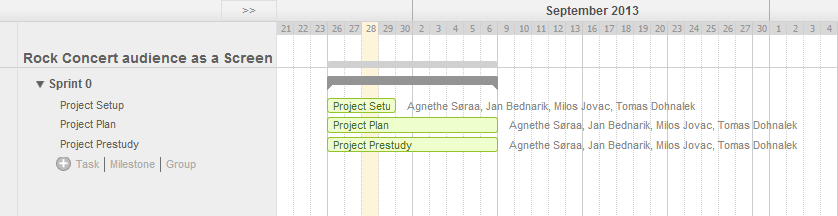
\includegraphics[scale=0.6]{images/gantt}
    \caption{Gantt Chart}
    \label{img:gantt}
\end{center}
\end{figure}

\subsection{Milestones}
\section{Risk managament}

\begin{table*}\centering \ra{1.3}
    \caption{Skills}
    \label{tab:skills}
    \vspace{2mm}
    \begin{tabular}{lcccc}
    \toprule
									
    \midrule
    \textbf{Event                	 } & Someone gets sick  		       & 1     & 2     & 3     \\ 
    \textbf{Consiquence              } & 4       					       & 1     & 1     & 1     \\ 
    \textbf{Possibility				 } & 5         						   & 1     & 4     & 1     \\ 
    \textbf{Risk                     } & 20        						   & 4     & 1     & 4     \\ 
    \textbf{Reactive Measures        } & Other people do more ours || Person can work from home         & 3     & 3     & 3     \\ 
    \textbf{Proactive Measures       } & Free weekends        			   & 3     & 1     & 2     \\ 
    \textbf{Responsible              } & All        					   & 2     & 5     & 1     \\ 
   
    \bottomrule
    \end{tabular}
\end{table*}

\begin{table*}\centering \ra{1.3}
    \caption{Skills}
    \label{tab:skills}
    \vspace{2mm}
    \begin{tabular}{lcccc}
    \toprule
                                & Agnethe   & Tomas & Milos & Jan \\
    \midrule
    \textbf{Leadership                 } & 4         & 1     & 2     & 3     \\ 
    \textbf{Scrum                      } & 4         & 1     & 1     & 1     \\ 
    \textbf{Mobile software development} & 3         & 1     & 4     & 1     \\ 
    \textbf{\LaTeX                     } & 1         & 4     & 1     & 4     \\ 
    \textbf{Network programming        } & 2         & 3     & 3     & 3     \\ 
    \textbf{Image processing           } & 1         & 3     & 1     & 2     \\ 
    \textbf{Java                       } & 3         & 2     & 5     & 1     \\ 
    \textbf{C++                        } & 1         & 4     & 3     & 4     \\ 
    \textbf{Testing                    } & 1         & 4     & 2     & 3     \\
    \bottomrule
    \end{tabular}
\end{table*}


\end{document}
